\chapter{Tecnologie nel dettaglio}
\section{Introduzione}
In questo capitolo andremo ad introdurre e analizzare alcune tecnologie che implementano i concetti riportanti nel capitolo precedente. Lo scopo di questo capitolo è quello di permettere al lettore di familiarizzare con alcuni concetti che poi saranno trattati nel prossimo capitolo.

\section{Gestione dei container: Docker}
Uno dei software disponibili per la gestione dei container, nonché uno dei più famosi, è Docker. Disponibile in forma gratuita, Docker è un progetto open source scritto interamente in Go e supportato da numerose aziende, come Google.

Abbiamo già discusso riguardo alla funzionalità e alla potenzialità dei container nel precedente capitolo. Grazie a Docker è possibile utilizzare i container anche su macchine che non utilizzano il kernel di GNU/Linux, in queste macchine viene creato uno strato aggiuntivo di virtualizzazione che permette all'applicativo di creare e gestire i container. Docker fornisce agli sviluppatori gli strumenti necessari per creare, gestire e configurare i container, tramite linea di comando o tramite un'interfaccia grafica.

\subsection{L'architettura di Docker}
L'architettura di Docker è basata sul tradizionale modello client-server.

\begin{figure}[h]
    \centering
    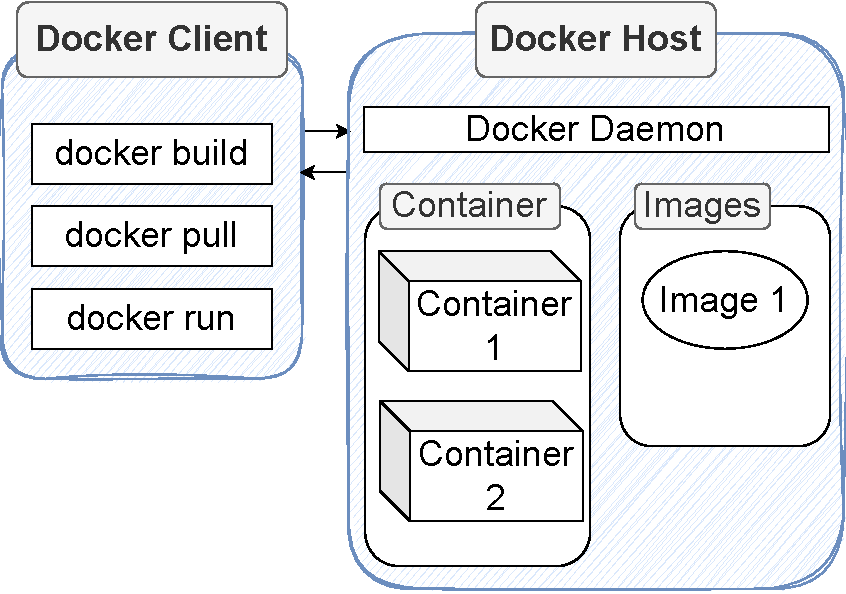
\includegraphics[scale=0.65]{capitoli/immagini/08_docker_architecture.pdf}
    \caption{Architettura di Docker}
    \label{fig:docker_arch}
\end{figure}

\paragraph{Docker Client}
Il docker client permette all'utente di interagire tramite interfaccia grafica o tramite riga di comando con il docker host. L'interfaccia grafica implementata in Docker però non permette di gestire tutte le componenti, l'utilizzo di Docker tramite riga di commando è consigliato anche dalla documentazione ufficiale. Di seguito sono riportati alcuni dei comandi più frequentemente usati:

\begin{enumerate}
    \item \textbf{\textcolor{color_1}{docker build -t <image\_name>}};
    \item \textbf{\textcolor{color_1}{docker pull <image\_name>}};
    \item \textbf{\textcolor{color_1}{docker run --name <container\_name> <image\_name>}};
\end{enumerate}

Il primo comando permette di creare un'immagine da un dockerfile \footnote{Un file di configurazione usato da Docker per la creazione di immagini.}, il secondo di scaricare un'immagine da Docker Hub \footnote{Il container register ufficiale di Docker \url{https://hub.docker.com/}.}. Il terzo comando permette la creazione di un container da un'immagine presente in locale, nel caso l'immagine non sia presente, Docker avviserà l'utente che dovrà eseguire il comando due per scaricare l'immagine richiesta.


\paragraph{Docker Host}
Il docker host rappresenta il cuore di Docker. Questo componente ha il compito di controllare i container. Per la definizione data in precedenza sappiamo che un container rappresenta una porzione del sistema operativo completamente isolata, allora ci chiediamo come sia possibile che i container, nella realtà, riescano a connettersi e scambiari informazioni tra di loro. Il kernel GNU/Linux non fornisce nessun meccanismo di dialogo tra container, ma Docker implementa una logica di networking per eliminare questo limite. L'implementazione delle regole di networking però rende le applicazioni che utilizzano i container meno sicure, durante la fase di sviluppo bisogna tener conto delle vulnerabilità scoperte sulle tecnologie utilizzate e correggerle. Per questo alcuni registri delle immagini permettono di effettuare delle scansioni sulle immagini e in caso di vulnerabilità notificare l'utente.

Di base tutti i file generati all'interno di un container vengono archiviati momentaneamente in un layer di persistenza dei dati, una volta che il container verrà distrutto (o terminato), i dati creati andranno perso. Docker implementa un meccanismo per rendere la persistenza dei dati definitiva, andando ad affidarsi alla macchina su cui docker host è in esecuzione. 

\begin{figure}[h]
    \centering
    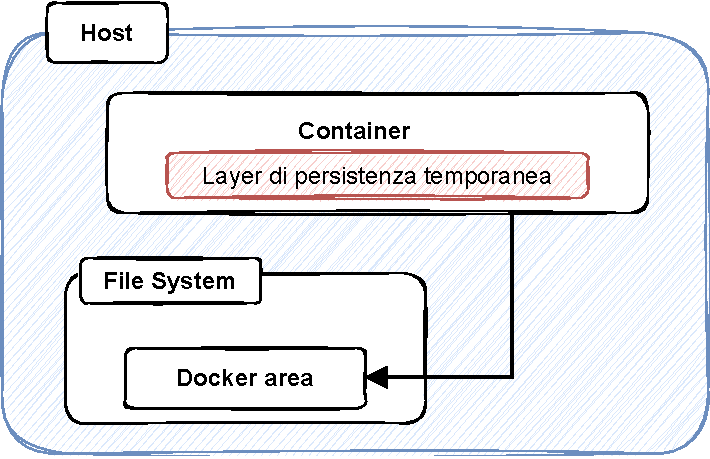
\includegraphics[scale=0.65]{capitoli/immagini/09_docker_volume.pdf}
    \caption{Persistenza dei dati in Docker}
    \label{fig:docker_persistance}
\end{figure}

Per semplicità consideriamo che Docker sia installato su una distribuzione del sistema operativo GNU/Linux, come possiamo osservare dalla figura sopra riportata, Docker implementa un meccanismo che permette ai container di dialogare col file system del computer host per accedere ad un'area di memoria, denominata docker area e creata durante l'installazione di Docker, e rendere persistenti i file creati durante l'esecuzione del container \footnote{In realtà Docker implementa altri due sistemi per la persistenza dei dati, il primo salva i dati generati in una qualsiasi posizione libera della memoria del computer host, il secondo metodo invece permette di depositare i dati nella memoria centrale, di fatto rendendoli temporanei.}. 

\section{Orchestrazione dei Container: Kubernetes}
Kubernetes \cite{K8S} è un software per l'orchestrazione dei container open source che  fornisce gli strumenti necessari per gestire i sistemi distribuiti in modo resiliente. Uno degli strumenti più importanti che Kubernetes implementa è il load balancer, alcune volte può presentarsi un eccessivo carico di lavoro su uno dei servizi, il load balancer permette una gestione automatica del carico di lavoro, in modo da non causare anomalie nel sistema.

Kubernets è un software che generalmente è disponibile tramite un servizio cloud, quando richiediamo un servizio del genere ciò che ci viene assegnato è chiamato un cluster. Di seguito possiamo osservare come funziona un cluster di Kubernetes:

\begin{figure}[h]
    \centering
    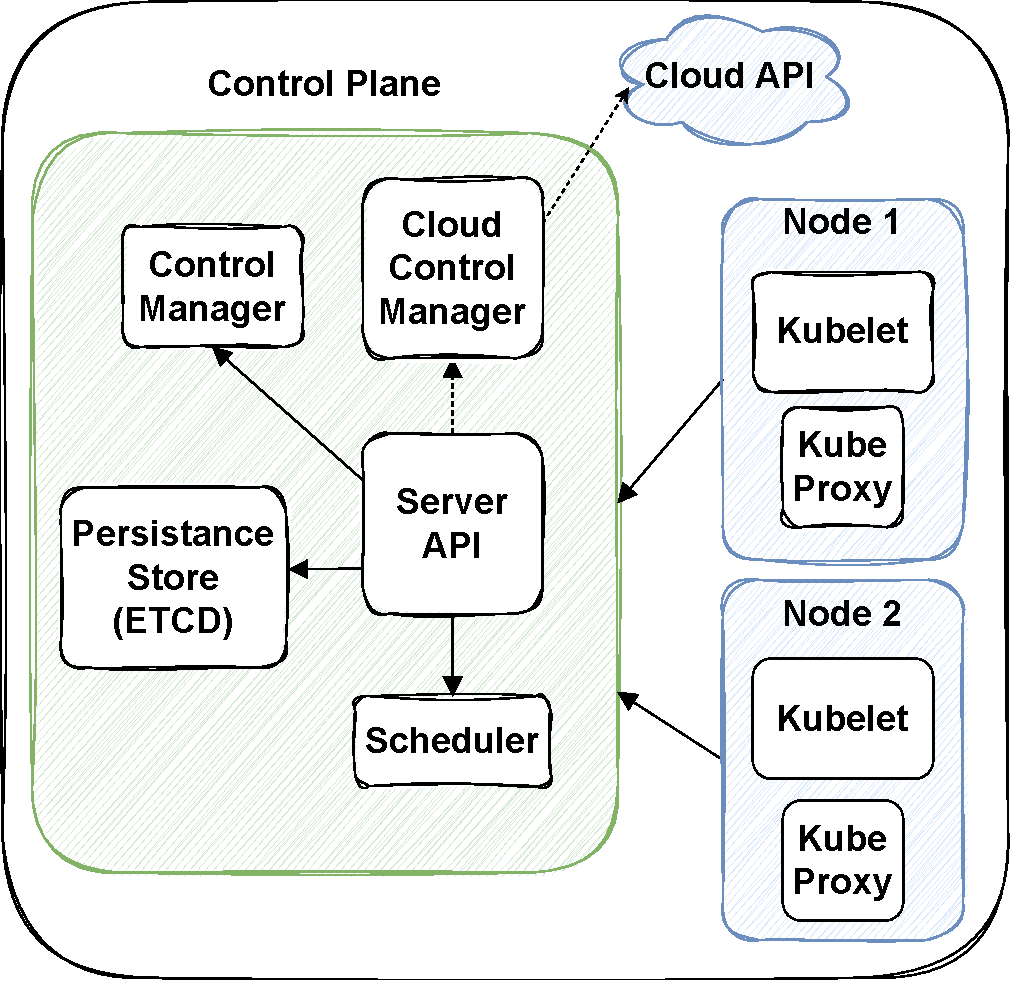
\includegraphics[scale=0.65]{capitoli/immagini/10_cluster_kubernetes.pdf}
    \caption{Cluster Kubernetes}
    \label{fig:Kubernetes_Cluster}
\end{figure}

\begin{comment}
\begin{itemize}
    \item Scoperta dei servizi e bilanciamento del carico;
    \item Orchestrazione dello storage; 
    \item Rollout e rollback automatizzati;
    \item Ottimizzazione dei carichi;
    \item Self-healing;
    \item Gestione di informazioni sensibili e della configurazione;
\end{itemize}
\end{comment}


\paragraph{Control Plane}
Il control plane è il componente principale di ogni cluster, mette a disposizione dell'utente tutte le funzionalità principali di Kubernetes. Il control plane può anche essere distribuito su più macchine.

\paragraph{Server API}
La prima componente che approfondiamo è il Server API. Il compito di questo componente è quello di esporre le API per accedere al control plane e poter controllare lo stato l'intero cluster. 

\paragraph{Persistance Store}
ETCD\footnote{Letteralmente /etc distributed.} è un software open source che si basa su concetto di rendere distribuita la cartella /etc presente nei sistemi operativi basati su Unix. In Unix la cartella etc contiene diversi file di configurazione. La componente integrata nel cluster di Kubernetes si occupa di rendere persistenti i file di configurazione utilizzando un sistema di chiave-valore e creando automaticamente dei backup sui dati ogni 30 minuti.

\paragraph{Scheduler}
Lo scheduler è quel componente del cluster che si occupa di gestire i nuovi pods assegnandoli ad uno dei nodi disponibile. Per pod si intende un gruppo di uno o più container che condividono le stesse informazioni di networking e di persistenza dei dati. Un pod rappresenta la più piccola unità che può essere creata e gestita da Kubernetes.

\paragraph{Controller Manager}
Il controller manager è formato da un insieme di processi che si occupano di gestire diverse parti del cluster. Un controller è un componente che  monitora costantemente lo stato del cluster tramite il server api e se lo stato desiderato non è quello attuale cerca di riportare il sistema ad uno stato precedente.

\paragraph{Cloud Controller Manager}
Esattamente come il controller manager, il cloud controller manager rappresenta un insieme di processi controller che si occupano di monitorare lo stato del cluster, ma solo di quelle componenti che gestiscono i processi cloud. Il cloud controller manager crea un collegamento tra il server API e la piattaforma di cloud scelta. Se per esempio si sceglie di utilizzare Kubernetes senza fare affidamento ad un servizio di cloud esterno, questa componente non farà parte del cluster.

\paragraph{Node}
Un nodo rappresenta un ambiente di runtime dove i container sono creati e gestiti.

\paragraph{Kubelet}
Processo che gestisce l'esecuzione dei container nei pod. Tale componente prevede l'esecuzione di diverse istruzioni che monitorano lo stato dei pod.

\paragraph{Kube-Proxy}
La rete condivisa tra container dello stesso pod viene gestita dalla componente nota come kube-proxy, inoltre permette ad un nodo di poter dialogare con gli altri nodi del cluster. L'implementazione base prevede l'utilizzo delle regole di networking del sistema operativo, ma è anche possibile che sia stesso la componente a gestire le comunicazioni.

\subsection{Orchestrazione in locale: minikube}
Kuberntes è un servizio accessibile principalmente via un servizio cloud. Generalmente tutti i più grandi cloud provider permettono di instanziare un cluster di Kubernetes. Essendo Kubernetes un software open source, la community ha reso disponibile un'implementazione in locale chiamata minikube. Tale software utilizza proprio Docker per emulare il funzionamento di Kubernetes.

\section{Gestione del Progetto: Apache Maven}
Una delle problematiche che affligge lo sviluppo moderno è la gestione delle dipendenze. Durante lo sviluppo di applicazioni è necessario fare affidamento su librerie esterne, per sopperire a mancate implementazione del linguaggio utilizzato. Una delle librerie esterne più utilizzate per lavorare con i file \ac{JSON} in Java è la libreria sviluppata da Google e mantenuta dalla comunità open source GSON. Java permette l'uso di librerie esterne a patto che il loro file sia incluso nel progetto. L'inclusione manuale delle librerie in Java però porta a diverse problematiche, sia con le librerie stesse, sia col coordinamento con il team di sviluppo, se il nostro progetto necessitasse di più librerie esterne dovremmo scaricare da Internet il file e poi includerlo nel nostro progetto e per ogni libreria dovremmo soddisfare, se presente, la catena di dipendenze, nel fare questo dovremmo anche informare il resto del team di sviluppo. 

Fortunatamente sono stati sviluppati software che si occupano di questo particolare aspetto (e non solo) della gestione del progetto. Apache Maven è uno di questi software ed è utilizzato principalmente in applicativi software basati su Java. Grazie a Maven la gestione delle dipendenze di un progetto diventa molto più semplice.

Maven non è uno strumento che gestisce solo le dipendenze di un progetto, permette anche di automatizzare la creazione del pacchetto e la possibilità di specificare una determinata struttura di progetto.

Il fulcro del software è un file chiamato \ac{POM}, scritto in \ac{XML}, tale file contiene tutte le istruzioni che necessità Maven per una corretta gestione del progetto. Nel pom sono presenti diverse informazioni, quelle più generiche che riguardano la versione, il nome, le informazioni sulla versione di Java utilizzata o altro, a quelle più specifiche come le dipendenze da soddisfare per il corretto funzionamento del software in sviluppo.

Maven permette anche di integrare dei plugin di terze parti, in questo modo è possibile creare degli strumenti per personalizzare il comportamento di Maven. Per esempio il framework Spring Boot integra il proprio plugin all'interno dei suoi progetti che utilizzano Maven.

\subsection{Un esempio di POM}

\paragraph{Introduzione del file}
Le prime righe di ogni file pom specificano la  versione della struttura e delle specifiche da seguire per quanto riguarda la scrittura dell'intero documento.
\begin{lstlisting}[language=XML, caption=Introduzione del POM]
<?xml version="1.0" encoding="UTF-8"?>
<project xmlns="http://maven.apache.org/POM/4.0.0"
	xmlns:xsi="http://www.w3.org/2001/XMLSchema-instance"
	xsi:schemaLocation="http://maven.apache.org/POM/4.0.0 https://maven.apache.org/xsd/maven-4.0.0.xsd">
	<modelVersion>4.0.0</modelVersion>
\end{lstlisting}


\paragraph{Informazioni del progetto}
Dopo le informazioni che riguardano il documento xml, abbiamo le informazioni che riguardano il progetto vero e proprio. 
\begin{lstlisting}[language=XML, caption= Informazioni del progetto che Maven deve gestire]
	<groupId>com.example.package</groupId>
	<artifactId>package</artifactId> <!-- Nome del pacchetto JAR/WAR -->
	<version>0.0.1-SNAPSHOT</version> <!-- Versione del pacchetto JAR/WAR -->
	<name>Nome del progetto</name>
	<description>Descrizione</description>
\end{lstlisting}
Come è possibile leggere in questa parte di xml vengono specificate le informazioni come nome del progetto, versione e descrizione. Queste informazioni sono utili a Maven durante la fase di creazione del pacchetto. Possono anche essere specificate delle proprietà, come per esempio la versione di Java utilizzata:
\begin{lstlisting}[language=XML, caption= Specifica della versione di Java]
	<properties>
		<java.version>11</java.version>
	</properties>
\end{lstlisting}


\paragraph{Dipendenze e Plugin}
Infine, il cuore del pom contiene tutte le informazioni per la gestione delle dipendenze e dei plugin. In questa parte di codice oltre a specificare quali plugin e quali dipendenze si intende utilizzare è anche possibile specificare ulteriore regole che Maven dovrà eseguire. Per esempio nei progetti in Java viene quasi sempre utilizzato il framework JUnit per effettuare dei test sull'applicativo in fase di sviluppo, questo pacchetto però non sarà più necessario quando l'applicazione sarà pronta per la distribuzione ed è possibile definire delle regole per escludere la dipendenza di JUnit quando Maven si occuperà di creare il pacchetto destinato al rilascio.
\begin{lstlisting}[language=XML, caption=Dipendenze e Plugin nel POM]
	<dependencies>
		<!-- Sezione dedicata alle dipendenze da soddisfare -->
	</dependencies>

	<build>
		<plugins>
			<!-- Sezione dedicata ai Plugin-->
		</plugins>
	</build>
</project>
\end{lstlisting}


\section{Framework: Spring Boot}
Uno dei framework più utilizzati per lo sviluppo back-end con il linguaggio di programmazione Java è sicuramente Spring Boot. La popolarità di questo framework lo rende una delle scelte migliori quando si decide di lavorare ad un applicazione che necessita di Java, grazie alla vasta utenza che ha deciso di includerlo nel propri progetti in rete è possibile trovare soluzioni di ogni tipo. Netflix è la principale sostenitrice del progetto Spring Boot, non solo aiuta nello sviluppo del framework, ma lo utilizza anche per il suo sistema basato sull'applicazione di streaming.

Spring Boot è basato sul framework Spring che a sua volta è basato sulle specifiche di Java Enterprise Edition. Il framework che stiamo esplorando ha 3 vantaggi principali:
\begin{enumerate}
    \item Configurazione automatica;
    \item Inversion of Control;
    \item Portabilità dell'applicativo;
\end{enumerate}

\paragraph{Configurazione automatica}
Le funzionalità implementate da Spring Boot sono operative dal momento della loro richiesta. Per esempio, se viene richiesta la componente di Spring Security, che come intuibile dal nome implementa i servizi per rendere sicura l'applicazione, una volta che la dipendenza sarà soddisfatta, Spring Boot assumerà il controllo per applicare a tale componente una configurazione di base, di fatto rendendola subito operativa.

Questo meccanismo non implica però che tale configurazione di base non possa essere modificata per implementare magari dei servizi aggiunti. Facendo riferimento sempre al caso di Spring Security, nessuno ci vieta di implementare un ulteriore sistema di autenticazione come \ac{JWT}.

Spring Boot permette di dover scrivere meno codice grazie alla configurazione automatica delle componenti, ma allo stesso tempo fornisce i meccanismi per configurare manualmente a nostro piacimento tale componente.

\paragraph{ Inversion of Control }
Il framework Spring Boot eredità da Spring due meccanismi: l'inversion of control e la dependency injection. 

Per inversion of control si intende quel meccanismo di ingegneria del software che trasferisce il controllo non più agli oggetti del nostro applicativo, ma al framework stesso. Nei linguaggi di programmazione tradizionali, come il C, noi facciamo uso delle librerie, con l'inversion of control il framework prende il controllo del flusso del nostro codice e quando richiesto lo richiama. 

I vantaggi dell'inversion of control sono diversi:
\begin{enumerate}
    \item disaccoppiamento dell'esecuzione di un servizio e la sua implementazione;
    \item facilità di implementazione di diverse soluzioni;
    \item facilità di testing dell'intero applicativo, grazie alla possibilità di isolare componenti e le loro dipendenza.
    \item una maggior modularià del programma;
\end{enumerate}
Per implementare l'inversion of control Spring utilizza il design pattern dependency injection.



\paragraph{Portabilità}
La portabilità è l'ultimo aspetto principale di Spring Boot. Questa funzionalità permette di creare un unico pacchetto con estensione \ac{WAR} del nostro applicativo, ma a differenza di un file WAR classico, Spring Boot rende il nostro pacchetto completo, pronto per il deployment.
